\documentclass[11pt,french]{report}
\usepackage[margin=0.7in,left=0.8in,right=0.8in]{geometry}
\usepackage[toc,page]{appendix}
\usepackage{graphicx}
\usepackage{natbib}
\usepackage{lipsum}
\usepackage{hyperref}
\usepackage[utf8]{inputenc}
\usepackage[T1]{fontenc}
\usepackage[french]{babel}
\usepackage{caption}
\usepackage[export]{adjustbox}
\usepackage[onehalfspacing]{setspace}
\usepackage{titlesec,xcolor}

\SetLipsumDefault{1}

\titleformat % design des titres des chapitres
{\chapter}
[display]
{\centering\normalfont\Large\scshape\bfseries}
{\rule[3pt]{0.15\linewidth}{3pt}\quad\chaptertitlename~\thechapter\quad \rule[3pt] {0.15\linewidth}{3pt}}
{0\baselineskip}%espace vertical entre chapitre et nom du chapitre
{\rule{\linewidth}{0.5pt}\break\Huge}
[\vspace{-0.5\baselineskip}\rule{\linewidth}{0.5pt}\vspace{0\baselineskip}]

\titlespacing{\chapter}{0}{0pt}{0pt}[0]

\begin{document}

\captionsetup[figure]{margin=1.5cm,font=small,labelfont={bf},name={Figure},labelsep=colon,textfont={it}}
\captionsetup[table]{margin=1.5cm,font=small,labelfont={bf},name={Tableau},labelsep=colon,textfont={it}}

\begin{titlepage}

\begin{center}

\par
\raisebox{-.5\height}{
\includegraphics[width=7cm]{images/LogoFSR}}
\hfill{}
\raisebox{-.5\height}{
\includegraphics[width=9cm]{images/LogoDXC}} 
\par
\vspace*{1.3cm}

\linespread{1.3}\huge {\bfseries Master Informatique :}\\\Huge{Traitement Inteligent des systèmes}

\rule{\textwidth}{2pt}\\[0.3cm]
\huge{\bfseries Rapport de stage de fin d'études}
\rule{\textwidth}{2pt}\\[0.3cm]

\linespread{1.5}\huge {\bfseries Intitulé :}\\
Conception et réalisation d'une application de gestion des effectifs en utilisant Microsoft Power Platform \\[0,3cm]

\linespread{1.3}\huge {\bfseries Fait par :}\\{\huge ARCHKAK Khalil}\\[0.5cm]

\noindent \Large{\textbf{soutenu le xx Septembre 2022 devant le Jury}} \\[0.7cm]

% \linespread{2}\huge{\bfseries Encadrant :}\\
% \large{- \textbf{Abdellah IDRISII:}}\normalsize{\textbf{Professeur au sein de la faculté de science de rabat et coordinateur du master IPS}}\\
% \large{- \textbf{Ahmed EL-YAHYAOUI :}}\normalsize{\textbf{Professeur au sein de la faculté de science de rabat}}

\begin{tabular}{lll}

\Large{M. Abdellah IDRISSI}  &  \Large{Professeur à la Faculté des Sciences  - Rabat} & \Large{\textit{Président}}	\\[0.1cm]
\Large{M. Ahmed EL-YAHYAOUI}   &  \Large{Professeur à la Faculté des Sciences - Rabat} & \Large{\textit{Encadrant}}	\\

\end{tabular}



% \begin{minipage}[t]{8cm}
% \linespread{2}\huge{\bfseries Encadrant :}\\
% \Large{\textbf{-} Abdellah IDRISSI}\\
% \Large{\textbf{-} Ahmed EL-YAHYAOUI}
% \end{minipage}
% \null\hfill
% \begin{minipage}[t]{6cm}
% \\[0.2cm]
% \linespread{2}\huge{\bfseries Maitre du stage :}\\
% \Large{\textbf{-} Adil EL-MESSARI}\\
% \end{minipage}
% \\[1.2cm]
\vspace*{1cm}
\linespread{1.3}\huge {\bfseries Réalisé le : \today}\\[0,3cm]
\textbf{\large{Année universitaire : 2021/2022}}

\end{center}

\end{titlepage}



% -------------------------------------------------------------------
% Abstract
% -------------------------------------------------------------------

\newgeometry{top=2cm,bottom=3cm,left=2.5cm,right=2.5cm}

\titleformat{\chapter}[display]
{\normalfont\huge\bfseries}{\filcenter\underline{\MakeUppercase{{\chaptertitlename}}\ \thechapter}}{20pt}{\Huge}

\titlespacing*{\chapter}{0pt}{1.80in}{0in}
\chapter*{\makebox[\linewidth]{Remerciements}}
\titlespacing*{\chapter}{0pt}{0.45in}{0.3in}%
\vspace{1in}

% Guidance of how to write an abstract/summary provided by Nature: https://cbs.umn.edu/sites/cbs.umn.edu/files/public/downloads/Annotated_Nature_abstract.pdf

Avant tout, je tiens à remercier ma mère, mon père, ainsi que mes deux frères pour leur soutien inconditionnel à la fois moral et économique, c’est  grâce à leur effort que je suis la aujourd’hui. \\

Je souhaite ensuite adresser mes profonds remerciements aux responsables et au personnel de la faculté de science de Rabat, spécialement à notre coordinateur du master \textbf{M. Abdellah Idrissi} pour la qualité de l’enseignement offert au sein de notre master ainsi que \textbf{M. Ahmed EL-YAHYAOUI} qui a toujours été à mon écoute. 
\\

Je souhaite également remercier tous les membres de l’équipe Power Platform de DXC Maroc, particulièrement \textbf{M. Adil El-MESSARI} qui a su me faire confiance lors de cette aventure dans le monde professionnel et a partagé ses connaissances de manière très pédagogique.\\ %Je le remercie aussi pour sa disponibilité et la qualité de son encadrement en entreprise.

Je voudrais enfin exprimer ma reconnaissance envers les amis et collègues qui m’ont apporté leur soutien moral et intellectuel tout au long de mon stage.




\titlespacing*{\chapter}{0pt}{1.80in}{0in}
\chapter*{\makebox[\linewidth]{ Résumé }}
\titlespacing*{\chapter}{0pt}{0.45in}{0.3in}%
\vspace{1in}

Ce rapport est le résultat du travail que j'ai réalisé dans le cadre de mon stage de fin d'études au sein de l'entreprise \textbf{DXC Technology Maroc}.\\

Le projet a comme objectif la conception et la réalisation d'une application de gestion des effectifs qui va aider l'entreprise à mieux gérer ses effectifs grâce à la construction d'une solution de bout en bout en utilisant la technologie Microsoft Power Platform qui permettra une meilleure visibilité, un meilleur suivi des personnels et être en mesure de déployer les bonnes ressources au bon moment.\\ 

Le présent rapport présente les différentes étapes de réalisation de cette application par lesquelles je suis passés dans le but de réaliser le travail qui m'a été confié. 

% -------------------------------------------------------------------
% Contents, list of figures, list of tables
% -------------------------------------------------------------------
% \newpage
% \tableofcontents

% \newpage
% \listoffigures


% -------------------------------------------------------------------
% Main sections (as required)
% -------------------------------------------------------------------

\newpage
\titlespacing*{\chapter}{0pt}{0in}{0.3in}
\chapter*{\makebox[\linewidth]{Introduction}}
\titlespacing*{\chapter}{0pt}{0.45in}{0.3in}%

Du 1er Mars 2022 au 1er septembre 2022 (6 mois), j’ai effectué un stage au sein de l’entreprise \textbf{DXC Technology Maroc} à Rabat. Au cours de ce stage j'ai pu acquérir de nouvelle compétence, de connaitre de nouvelles technologies au-delà de ceux apprise lors de ma formation master et de surtout m'immerger dans le monde professionnel. \\ 

\textbf{DXC Technology Maroc} est une entreprise de technologie dont le siège se trouve dans la technopole de Rabat, Technopolis. Il s’agit d’une coentreprise du groupe \textbf{DXC Technology} et de la \textbf{Caisse de dépôt et de gestion du Maroc}. \textbf{DXC Technology Maroc} a pour vocation d’accompagner les très grands donneurs d’ordre publics et privés dans leur transformation digitale au niveau de plusieurs service : Data Center, Cloud et Platform, BI Analytics, Sécurité, Service applicatif, Modern Workplace, Business Process et Conseil.\\ 

Mon stage au sein de \textbf{DXC Technology Maroc} a consisté essentiellement en la conception d'une application de gestion d'effectifs. Tout d'abord on a commencé par l'identification des besoins, ensuite la création de la feuille de route du produit, Puis la création de l'expériences utilisateur avec un design soigné et puis à partir de là, commencez à développer le backend, par la suite la validation de la qualité de l'application avec une série de test pour finalement déployer l'application, la documenter, et recueillir les commentaires. Plus largement, ce stage a été l’opportunité pour moi d'accéder au monde professionnel. Au-delà du fait d’enrichir mes connaissances en \textbf{Buisness Inteligence}, ce stage m’a permis de comprendre à quelle point la suite \textbf{Microsoft Power Platform} peut faciliter la transformation digitale avec un environnement “Low-Code” voire “No-Code” qui permet de diminuer les différentes étapes de développement d'une application et de production de quelque mois a quelques semaines.\\

Pour présenter mon expérience de stage au sein de la société \textbf{DXC Technology Maroc}, nous nous intéresserons à la description générale de l’entreprise et le contexte général du projet (Chapitre 1), puis nous nous pencherons a une étude générale du projet (Chapitre 2), ensuite l’étude des besoins décrivant les contraints et l’étude fonctionnels du projet (Chapitre 3), Par la suite la solution technique, les outils de développement avec lequel j’ai travaillé durant ces 6 mois à savoir Microsoft Power Platform (Chapitre 4), pour finalement présenter la partie de réalisation du projet qui contient les captures des écrans des interfaces les plus pertinentes du projet (Chapitre 5).


\newpage
\titleformat % design des titres des chapitres
{\chapter}
[display]
{\centering\normalfont\Large\scshape\bfseries}
{\rule[3pt]{0.15\linewidth}{3pt}\quad\chaptertitlename~\thechapter\quad \rule[3pt] {0.15\linewidth}{3pt}}
{0\baselineskip}%espace vertical entre chapitre et nom du chapitre
{\rule{\linewidth}{0.5pt}\break\Huge}
[\vspace{-0.5\baselineskip}\rule{\linewidth}{0.5pt}\vspace{0\baselineskip}]

\let\clearpage\relax% Stop LaTeX from going to a new page; and
\vspace*{5.5cm}%

\chapter{Context general du projet}
Dans ce premier chapitre, je vais présenter l’entreprise d’accueil
DXC Technology Maroc à travers une description de l’historique ainsi
que son domaine d’activité et l’organigramme puis enfin une
présentation de ses clients.




\newpage
\section{Organisme d’accueil}
\subsection{Présentation de DXC Technology}

\begin{wrapfigure}{l}{0.42\textwidth}
  \begin{center}
    
\includegraphics[width=0.4\textwidth]{Rapport de stage PFE chez DXC/images/LogoDXC.png}
  \end{center}
\end{wrapfigure}
\\
HP-CDG IT Services Maroc est le fruit d’un partenariat stratégique
entre HPE (Hewlett Packard Enterprise), leader mondial du marché IT
et CDG (la Caisse de Dépôt et de Gestion)
\\
\\

Créée en 2007, HP-CDG IT Services Maroc a pu se positionner
rapidement parmi les acteurs leaders du conseil, des services informatiques et de
l’infogérance en profitant de l’expertise mondialement reconnu de HP. Ils développent
aujourd’hui une large gamme de conseils, de solutions et de services technologiques.
\\
\\
Précédemment connue sous le nom HP CDG IT Services Maroc, DXC Technology au Maroc est
née suite à un partenariat entre DXC Technology et la Caisse de Dépôt et de Gestion, cette nouvelle dénomination a pris effet le 3 Avril 2017 suite à la naissance de DXC Technology à travers une fusion entre Hewlett Packard Enterprise (HPE) et Computer Sciences corporation (CSC).
\\
\\
Cette fusion ayant donné naissance à l’un des plus gros acteurs de services aux entreprises au monde : DXC Technology, ce nouveau Groupe dispose d’un portefeuille de plus de 5900 clients répartis dans plus de 70 pays, dont le Maroc.
\\
\\
DXC Technology a été créée sur des fondations solides de confiance et de transformation et sur l’ambition renouvelée d’aider les clients à prospérer par le changement Digital. Ainsi, ils sont reconnus comme un multiplicateur de forces avec l’objectif principal d’apporter plus de valeur aux clients, aux partenaires et aux actionnaires de la société, et d’offrir davantage d’opportunités aux collaborateurs du groupe.
\\
\\
DXC Technology Maroc bénéficie de plus de 15 ans d’expérience dans le domaine informatique comptant plus de 1200 collaborateur qui travaille aujourd’hui en deux modes : hybride et distancielle.

\newpage
\subsection{Fiche signalétique de l’entreprise }

Le tableau suivant présente la fiche signalétique de l’entreprise, c’est la carte d’identité de
l’entreprise.

\begin{figure}[h]
    \centering
    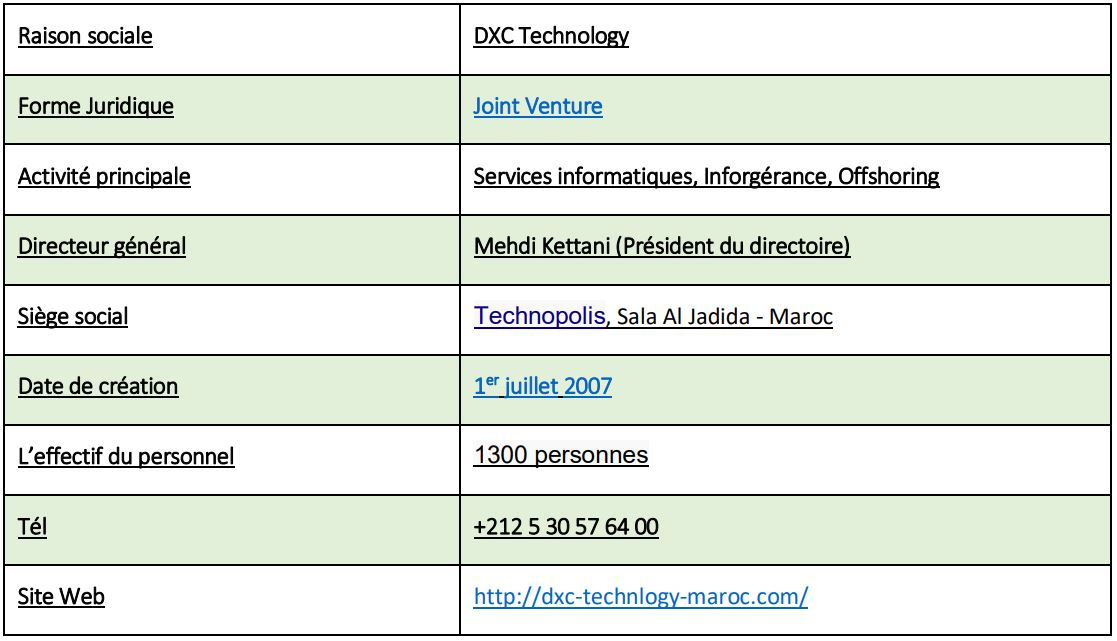
\includegraphics[width=\textwidth]{Rapport de stage PFE chez DXC/figures/fiche_entreprise.jpg}
    \caption{Fiche signalétique de l'entreprise}
\end{figure}

\newpage

\subsection{Historique et fait Marquants }

La figure suivante présente l’évolution d’aventure de l’entreprise depuis 2007 jusqu’à 2014.

\begin{figure}[!h]
    \centering
    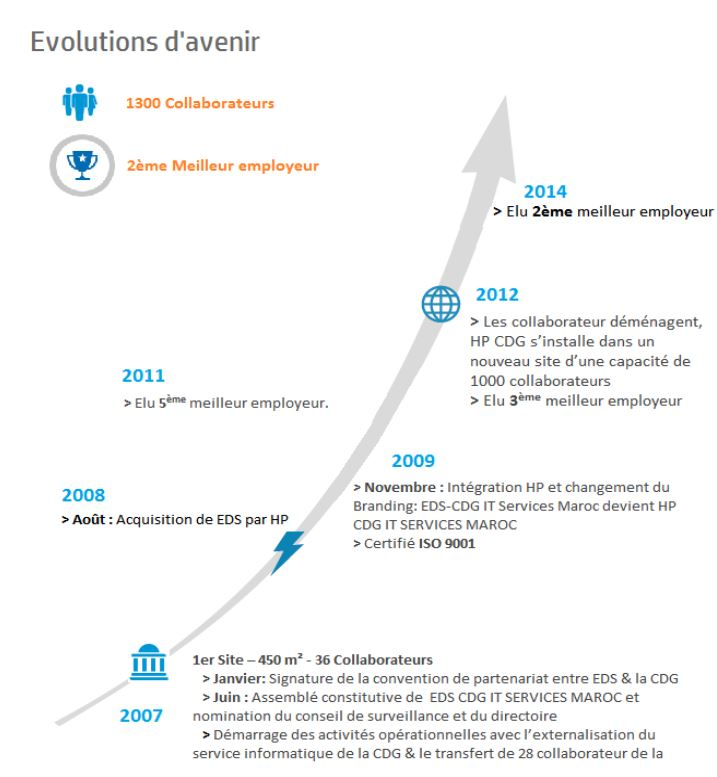
\includegraphics[scale=0.9,keepaspectratio]{Rapport de stage PFE chez DXC/figures/evolution_entreprise.jpg}
    \caption{Evolution de DXC Technology Maroc}
\end{figure}

\newpage
\subsection{DXC Technology histoire de succès }

La figure suivante présente l’histoire de succès de l’entreprise DXC Technology et l’évolution du nombre des employés depuis 2007

\begin{figure}[!h]
    \centering
    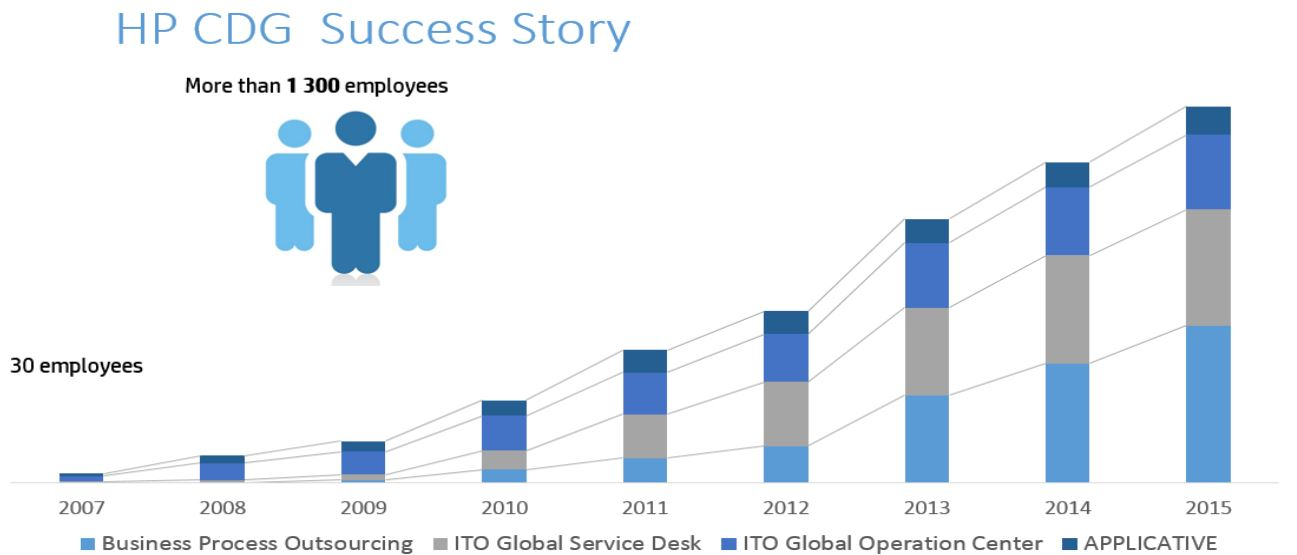
\includegraphics[scale=0.5,keepaspectratio]{Rapport de stage PFE chez DXC/figures/sucess_story.jpg}
    \caption{Histoire de succès de DXC Technology}
\end{figure}

\subsection{Secteurs d’activités}

DXC Maroc délivre un large evantail de compétence :

\begin{figure}[!h]
    \centering
    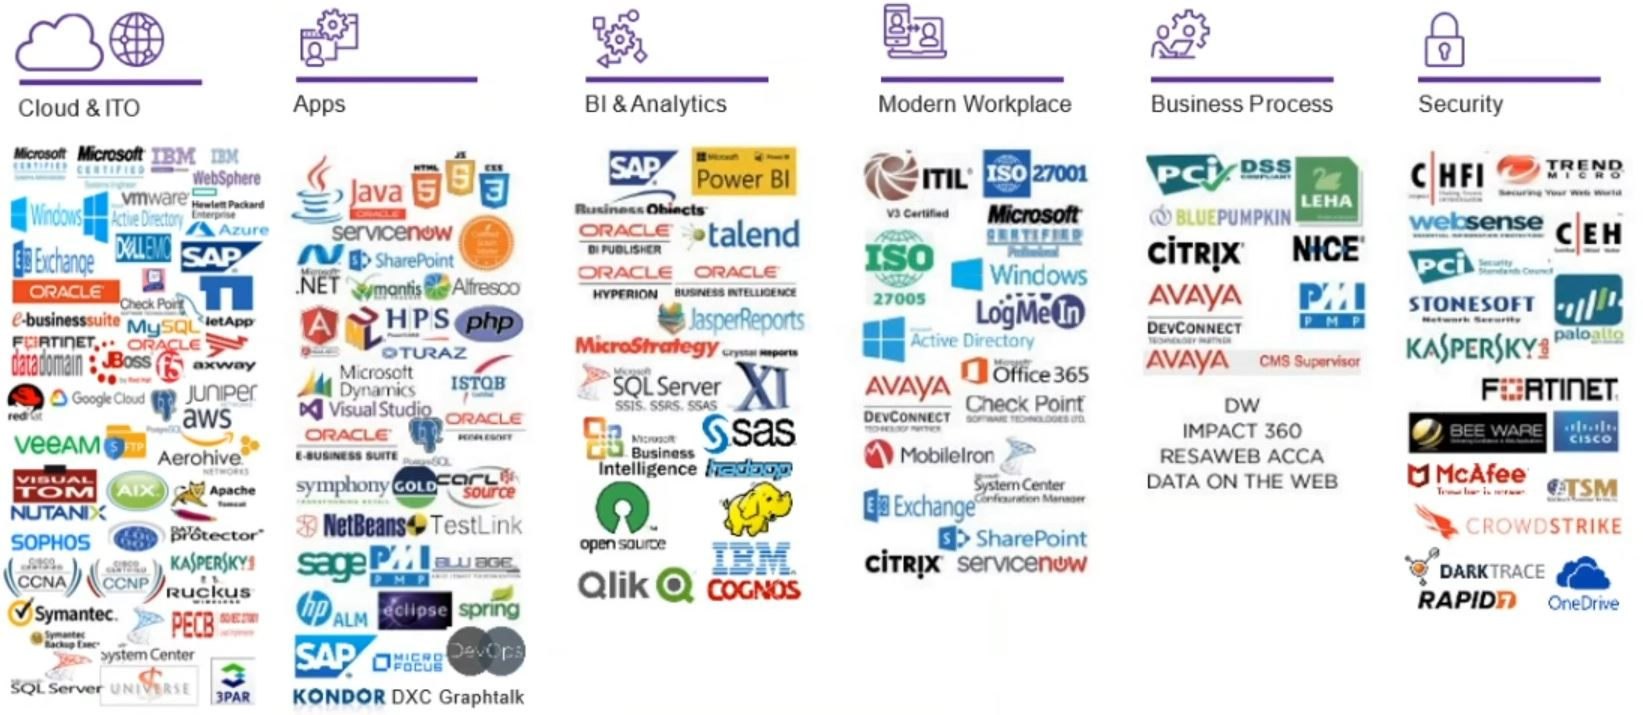
\includegraphics[scale=0.4,keepaspectratio]{Rapport de stage PFE chez DXC/figures/competence.jpg}
    \caption{Les clients de DXC Technologie Maroc}
\end{figure}

\newpage
DXC Technology est un centre de services qui dispose de ressources compétentes dans les
métiers de services informatiques suivants :

\begin{description}
  \item \textbf{Assurance:} La première mondiale des services et des solutions logicielles pour l’assurance. Soutient la croissance des assureurs, et amélien leur time-to-market et leur excellence opérationnelle grâce à des solutions d’assurance digitale et de gestion déléguée de leurs processus métiers.
  \item \textbf{Sante et Sciences de la vie:} Elle propose des logiciels leaders sur le marché et des services de gestion déléguée (BPS) pour les fournisseurs de soins, les payeurs, l’Etat et les entreprises de soins de santé. Elles se focalisent sur les soins cliniques et l’efficacité opérationnelle avec ses solutions de transformation digitale de soins.
  \item \textbf{Secteur public:} Ils sont un des leaders mondiaux de services informatiques indépendants et travaillent à tous les niveaux (Etat, administrations, collectivistes locales). Ils proposent pour les opérations et systèmes critiques une assistance 24 heures sur 24, et 7 jours sur 7.
  \item \textbf{Énergie:} Depuis plus de 20 ans, ils ont accompagné plus de 400 acteurs du secteur énergétique dans le monde entier. Leurs solutions les aident à saisir rapidement les opportunités du marché, se forger un avantage concurrentiel et mettre en œuvre de nouveaux modèles économiques.
  \item \textbf{Énergie:} Ils sont un desacteurs principaux des services informatiques dédiés aux secteurs Automobile, Équipements industriels, Chimie et High Tech. Ils allaient leurs solides connaissances sectorielles à des expertises spécifiques (Internet des objets, analytique, sécurité) pour aider leurs clients à doper leur innovation.
  \item \textbf{Communication, médias et divertissement:} Ils fournissent des solutions métiers innovantes aux acteurs du secteur Communication, médias et divertissement, aux quatre coins du monde, pour les aider à transformer leur organisation, réenchanter l’expérience client et tirer profit de la convergence digitale.
  \item \textbf{Aéronautique et défense:} Ils sont un des leaders des services informatiques dédiés au secteur Aéronautique et défense. Ils aident leurs clients à raccourcir leur time-to-market, prendre de meilleures décisions en exploitant la richesse de leurs données et adopter les technologies digitales. Ils accélèrent la mise en œuvre de l’innovation sur l’ensemble de la chaîne d’approvisionnement et de fabrication.
  \item \textbf{Transport et tourisme:} Avec plus de 40 ans d’expérience sur le marché, elle soutient les systèmes critiques du secteur (compagnies aériennes, passagers, fret, logistique, entreprises ferroviaires). Ses services aident leurs clients à soutenir leur croissance et les accompagne durant leur transformation.
  \item \textbf{Industrie:} Ils sont un desacteurs principaux des services informatiques dédiés aux secteurs Automobile, Équipements industriels, Chimie et High Tech. Ils allaient leurs solides connaissances sectorielles à des expertises spécifiques (Internet des objets, analytique, sécurité) pour aider leurs clients à doper leur innovation.
  \item \textbf{Distribution et grande consommation:} Ils aident les leaders mondiaux de la distribution et des biens de grande consommation se concentrer sur l’expérience client, et à saisir les opportunités liées aux nouvelles tendances digitales.
  \item \textbf{Communication, médias et divertissement:} Ils fournissent des solutions métiers innovantes aux acteurs du secteur Communication, médias et divertissement, aux quatre coins du monde, pour les aider à transformer leur organisation, réenchanter l’expérience client et tirer profit de la convergence digitale.
  \item \textbf{Aéronautique et défense:}Ils sont un des leaders des services informatiques dédiés au secteur Aéronautique et défense. Ils aident leurs clients à raccourcir leur time-to-market, prendre de meilleures décisions en exploitant la richesse de leurs données et adopter les technologies digitales. Ils accélèrent la mise en œuvre de l’innovation sur l’ensemble de la chaîne d’approvisionnement et de fabrication.
  
\end{description}

\subsection{Les clients de DXC Technologie Maroc }

La figure suivante présente les différents clients et partenaires commerciaux de DXC.

\begin{figure}[!h]
    \centering
    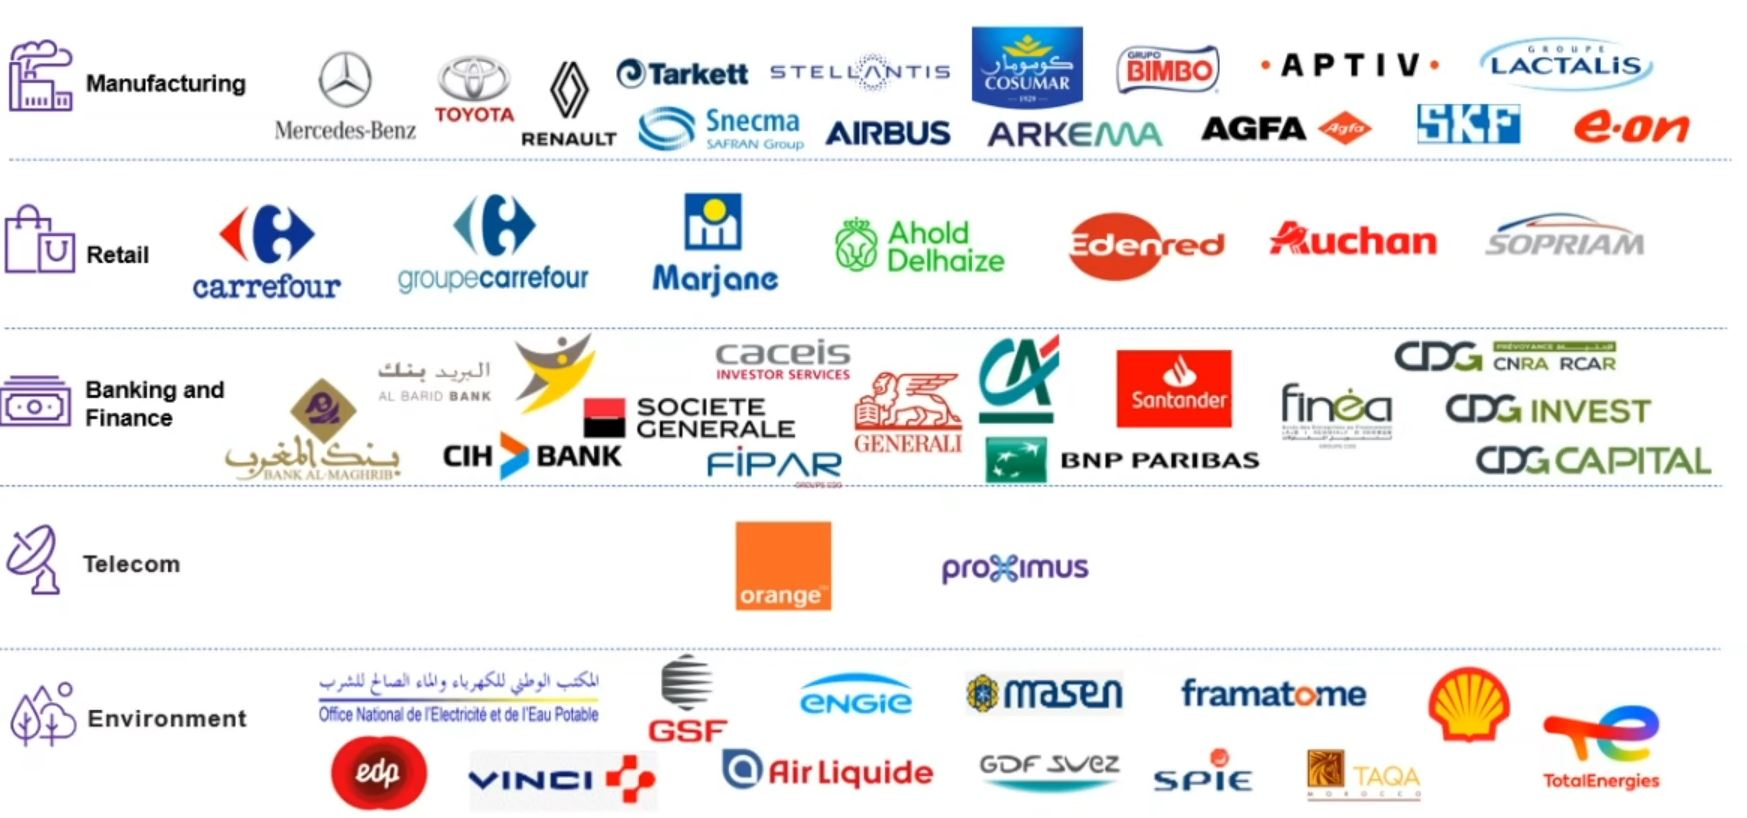
\includegraphics[scale=0.36,keepaspectratio]{Rapport de stage PFE chez DXC/figures/client.jpg}
    \caption{Les clients de DXC Technologie Maroc}
\end{figure}

\newpage
\subsection{Organigramme }
La figure suivante présente quelques divisions principales de l’entreprise et pas la totalité
des divisions, il est divisé en 2 parties "Support" et "Services Lines" :

\begin{description}
  \item \textbf{Support :} rassemble l’ensemble d'activités de gestion considérées comme ne constituant pas le cœur de métier. Ces activités assurent le fonctionnement de l'entreprise et sont généralement communes à plusieurs divisions ou ligne de produits métier, tel que le service Finance, Ressources Humaines, marketing et service de ventes.
  \item \textbf{Service Lines :} contient les divisions qui représentent le cœur de métier, ces divisons
 sont :
 \begin{enumerate}
   \item \textbf{Application Services :} représente généralement les services de développement informatique et qualité logiciel, ainsi que l’intégration des ERP et le support applicatif.
   \item \textbf{Global Operations Services :} c’est une division dédiée pour les services d’Infrastructure, Cloud et Sécurité des systèmes d’information.
   \item \textbf{Business Process Outsourcing : } l’ensemble des activités qui ont comme but l'externalisation d'une partie de l'activité de l'entreprise vers un prestataire extérieur.
    \item \textbf{MWS  : } assure les services de gestion et support de mobilité, et le support au Delivery.
 \end{enumerate}
  
  \begin{figure}[!h]
    \centering
    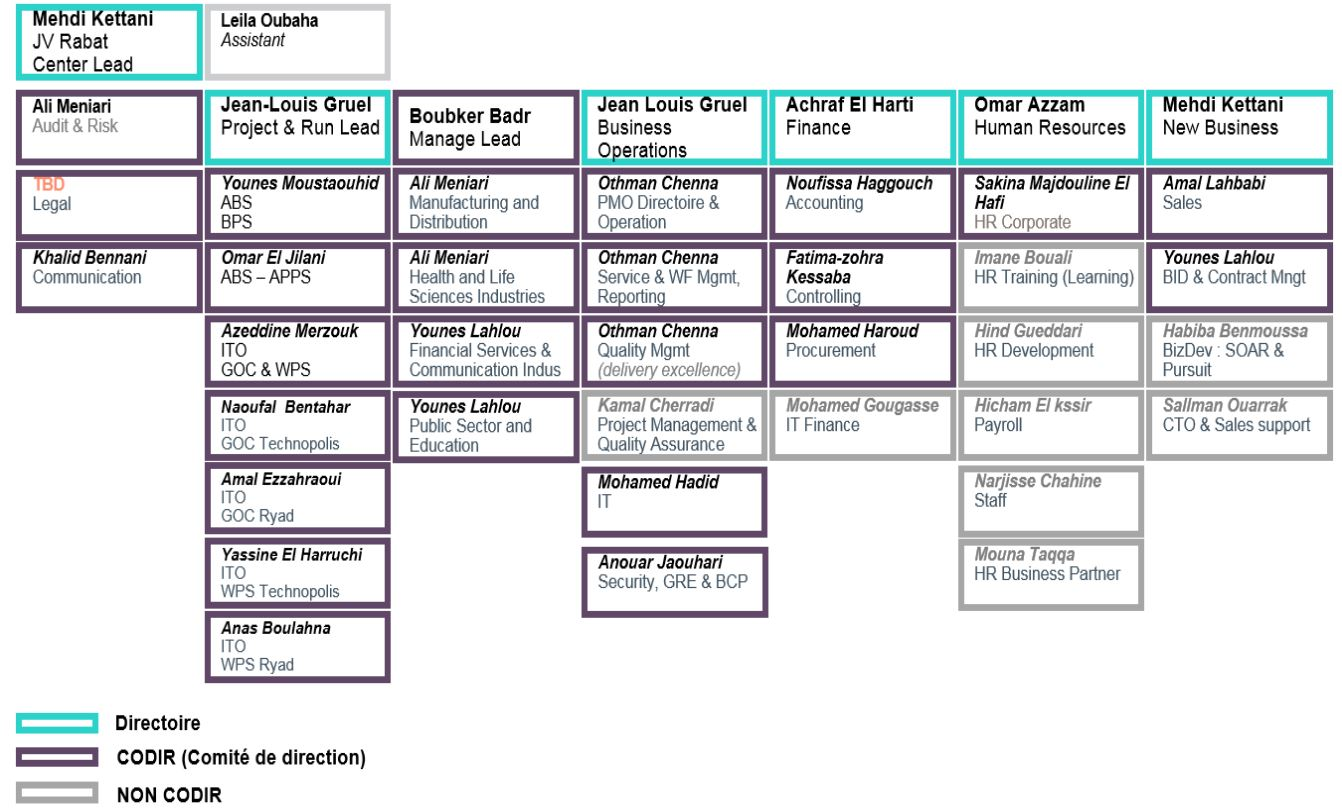
\includegraphics[scale=0.5,keepaspectratio]{Rapport de stage PFE chez DXC/figures/organigramme.jpg}
    \caption{Organigramme de DXC Technology}
\end{figure}
  
\end{description}

\subsection{Les Certification }

Cette figure montre les differentes certification que possede DXC Technology Maroc : 

\begin{figure}[!h]
    \centering
    
\includegraphics[scale=0.4,keepaspectratio]{Rapport de stage PFE chez DXC/figures/certifications_dxc.jpg}
    \caption{Certification de DXC Technology Maroc}
\end{figure}

\section{Cadre général du projet }
Vue le besoin qu’a déclaré le service financier de \textbf{DXC Technologie Maroc}, les responsables du service Line APPS ont été obligé de construire une équipe pour commencer la planification, l’étude ainsi que le développement du projet dont j’ai été affecté. Ce besoin a été créé à cause du traitement manuel des données de la gestion des Pipes et les appels d’offres ainsi que la construction des équipes et l’affectation des ressources pour chaque équipe. La digitalisation de ce processus permettra de passer d'une méthodologie qui prenais en compte plusieurs fichier Excel partageais sur plusieurs teams en une application \textbf{Power App} qui regroupera toutes les informations nécessaires de façon homogène.


\section{Conclusion}
Dans ce chapitre j’ai présenté l’organisme d’accueil, puis situé le projet dans son contexte général. Le chapitre suivant se concentrera sur l’étude générale du projet.


\newpage
% \input{sections/results.tex}
% \input{sections/discussion.tex}
% \input{sections/conclusion.tex}


% -------------------------------------------------------------------
% Bibliography
% -------------------------------------------------------------------

% \bibliographystyle{agsm} 
% \bibliography{mybibliography} 


% -------------------------------------------------------------------
% Appendices
% -------------------------------------------------------------------

% \begin{appendices}
% % \input{sections/appendixA.tex}
% % \input{sections/appendixB.tex}
% \end{appendices}

\end{document}
